\documentclass[a4paper,12pt]{article}
\usepackage[T1]{fontenc}
\usepackage[utf8]{inputenc}
\usepackage[italian]{babel}
\usepackage{lmodern}

\usepackage{enumitem}
\usepackage{commath}
\usepackage{bbold}
\usepackage{physics}
\usepackage{amsmath}
\usepackage{amsfonts}
\usepackage{amssymb}
\usepackage{amsthm}
\usepackage{graphicx}
\usepackage[colorinlistoftodos]{todonotes}
\PassOptionsToPackage{hyphens}{url}
\usepackage[colorlinks=true, allcolors=blue]{hyperref}
\usepackage{siunitx}
\sisetup{separate-uncertainty=true}
\usepackage{footnotebackref}
\usepackage{framed}
\usepackage{thmtools}
\usepackage{etoolbox}
\usepackage{fancybox}
\usepackage{slashed}
\newcommand{\DD}{\mathrm{D}}
\usepackage{mathrsfs}

\newenvironment{myleftbar}{%
\def\FrameCommand{\hspace{0.6em}\vrule width 2pt\hspace{0.6em}}%
\MakeFramed{\advance\hsize-\width \FrameRestore}}%
{\endMakeFramed}
\declaretheoremstyle[
spaceabove=6pt,
spacebelow=6pt
headfont=\normalfont\bfseries,
headpunct={} ,
headformat={\cornersize*{2pt}\ovalbox{\NAME~\NUMBER\ifstrequal{\NOTE}{}{\relax}{\NOTE}:}},
bodyfont=\normalfont,
]{exobreak}

\declaretheorem[style=exobreak, name=Esercizio,%
postheadhook=\leavevmode\myleftbar, %
prefoothook = \endmyleftbar]{exo}

\newcommand{\boxalign}[2][0.986\textwidth]{
  \par\noindent\tikzstyle{mybox} = [draw=black,inner sep=6pt]
  \begin{center}\begin{tikzpicture}
   \node [mybox] (box){%
    \begin{minipage}{#1}{\vspace{-5mm}#2}\end{minipage}
   };
\end{tikzpicture}\end{center}}

\usepackage{alumnistem}

\author{Jacopo Tissino}
\title{Indivisibilità del fotone alla STEM Academy}
\date{Luglio 2020}

\usepackage[
backend=biber,
style=alphabetic,
sorting=nyt,
backref=true
]{biblatex}

\addbibresource{STEM_Indivisibility.bib}

% \title{L'indivisibilità del fotone: Summer STEM Academy 2020}

\begin{document}

\maketitle

\tableofcontents

\medskip

Iniziamo con un quiz: \textbf{cos'è la luce}?

\begin{enumerate}[label=\emph{\alph*})]
    \item Un'onda.
    \item Una particella.
    \item Sia un'onda che una particella. 
    \item Né un'onda né una particella. 
    \item A volte un'onda, a volte una particella.
    \item Mi astengo.
\end{enumerate}

La domanda, posta in questo modo vago (e provocatorio), rischia di allontanarsi dall'ambito di ricerca della Fisica: non siamo generalmente interessati a descrivere l'\emph{essenza fondamentale} di un oggetto, bensì cerchiamo di fornire modelli che ne descrivano il comportamento e che siano in grado di predire i risultati degli esperimenti che facciamo. 
Questo approccio all'investigazione spesso riesce a darci grande chiarezza sul come pensare agli oggetti fisici. 

% TODO keep this bit?

Tenendo questo in mente, cerchiamo di rispondere alla domanda.
Innanzitutto, dobbiamo chiarire qual'è l'oggetto fisico che vogliamo descrivere.

Partiamo dalla descrizione più intuitiva: la luce è quello che vediamo con gli occhi. 
Vedremo che, investigando questo fenomeno nel dettaglio, questa definizione risulterà restrittiva e ci porterà a ridefinire quella che vediamo con gli occhi come \emph{luce visibile} --- quindi, c'è anche della ``luce invisibile''.

Per ora, tuttavia, partiamo dalle prime teorie della luce, che volevano descrivere solo quella visibile.

\section{Teorie della luce}

\subsection{Newton versus Huygens} \label{sec:newton-vs-huygens}

Lo storico dibattito è quello fra Newton e Huygens. 

Newton (1642--1726/1727), il più famoso dei due, proponeva una \textbf{teoria corpuscolare} della luce. 

Secondo questa teoria, la luce è composta di corpuscoli molto leggeri che viaggiano ad una velocità finita. 

Quali fenomeni voleva spiegare Newton con questa teoria?
Riflessione e rifrazione, innanzitutto: lui ha dimostrato che facendo passare la luce per un prisma si può scomporla nelle sue componenti cromatiche, e --- qui la chiave! --- questo processo è reversibile: con un altro prisma è possibile ricomporre la luce bianca.

La luce, dunque, viene deviata quando passa per un'interfaccia, e di quanto viene deviata dipende dal suo colore. 

La riflessione invece è ciò che accade per uno specchio: la luce ``rimbalza'' ad un angolo uguale a quello di incidenza.

La teoria di Newton ha delle spiegazioni per questi fenomeni, seppur non completamente soddisfacenti.
Newton la mette in pratica per costruire telescopi: il telescopio Newtoniano utilizza solo specchi invece che lenti, eliminando quindi l'aberrazione cromatica che le caratterizza. 

La teoria corpuscolare ha dietro l'apparato della nuovissima meccanica Newtoniana: la luce viene descritta come un insieme di piccole particelle con massa molto ridotta (o nulla? al tempo  di Newton non c'era davvero modo di determinarlo) che si muovono molto velocemente rispettando le leggi di Newton: inerzia, \(\vec{F} = m \vec{a}\) e azione-reazione.

Un vantaggio della teoria corpuscolare è il fatto che non richiede un \emph{etere luminifero} (portatore della luce). 

La teoria di Huygens è \textbf{ondulatoria}: vede la luce come un'onda che si propaga in un qualche tipo di etere, in modo simile a come si comportano le onde nell'acqua poco profonda.

Questa teoria spiega, al contrario di quella corpuscolare, il fatto che all'interfaccia fra due mezzi ci siano sia riflessione che rifrazione: nella meccanica ondulatoria questo è un fatto naturale e atteso.

Nel contesto della meccanica ondulatoria, si può derivare la legge di Snell, che governa l'angolo al quale la luce viene diffratta. 

Iniziamo però con i preliminari della teoria ondulatoria: guardiamo il caso monodimensionale per semplicità, guardare il problema in più dimensioni è utile ed interessante ma le caratteristiche principali si possono evincere già da qui. 

La caratteristica principale delle onde è la periodicità: partiamo da quella che si chiama onda \emph{monocromatica}, il caso più semplice, che ha un periodo ben definito.
Le equazioni che ora scriviamo potrebbero descrivere, ad esempio, la variazione del livello dell'acqua lungo una linea che tracciamo in uno stagno: chiamiamola \(A\).
\(A\) può assumere un valore positivo o negativo, se vale 0 significa che il livello è quello che avrebbe lo stagno senza perturbazioni.

Se fissiamo un istante temporale \(t_0 \) e ``fotografiamo'' l'onda, la formula che la descrive è 
%
\begin{align}
\eval{A(x)}_{t = t_0 } = A_0 \sin(2 \pi \frac{x}{\lambda } +\varphi )
\,.
\end{align}

\(A_0 \) è l'ampiezza massima che raggiunge l'onda, l'altezza dei picchi e la profondità delle valli. \(\lambda \) è una lunghezza caratteristica dell'onda, detta \emph{lunghezza d'onda}: è la distanza fra due picchi vicini, o fra due valli vicine; se \(x\) --- la posizione spaziale lungo la linea --- varia aumentando o diminuendo di esattamente \(\lambda\) l'ampiezza non cambia.
Questo è dovuto al fatto che la funzione seno ha una periodicità di \(2 \pi \). 

Il termine \(\varphi \) si chiama \emph{fase}, ed esprime il fatto che nel punto che chiamiamo \(x=0\) l'onda può essere in un massimo, un minimo, o a qualunque punto della sua evoluzione. 
Visto che \(\varphi \) è arbitrario, è arbitraria anche la scelta di un seno piuttosto che un coseno: cambiando \(\varphi \) di \(\pi /2\) possiamo passare dall'uno all'altro. 

Se vogliamo includere la dipendenza dal tempo, otterremo una formula di questo tipo: 
%
\begin{align}
A(x, t) = A_0 \sin(2 \pi \qty( \frac{x}{\lambda } - \frac{t}{T}) + \varphi )
\,.
\end{align}

Abbiamo inserito un tempo caratteristico \(T\), chiamato \emph{periodo}: se fissiamo la posizione \(x\) e guardiamo solo un punto, l'onda torna al punto dov'era prima dopo un tempo \(T\). 
C'è un meno perché stiamo assumendo che l'onda avanzi verso destra, ovvero verso le \(x\) positive: se \(x\) aumenta di un poco, per mantenerci nella stessa posizione (``viaggiando con l'onda'', ovvero tornando allo stesso valore dell'argomento del seno) dobbiamo aumentare un poco anche \(t\), ovvero aspettare un poco. 

Questo è il caso \emph{monodimensionale}; se abbiamo un'onda in due o tre dimensioni spaziali che si propaga lungo l'asse \(x\) avrà esattamente la stessa forma; invece di una cresta avremo un \emph{fronte d'onda} lungo il quale il seno ha lo stesso valore. 
Il vettore che definisce la direzione nella quale l'onfa si propaga è detto \emph{vettore d'onda}, nel nostro caso sarebbe parallelo all'asse \(x\) e dunque perpendicolare al fronte d'onda. Convenzionalmente lo si prende di modulo pari a ciò che moltiplica \(x\) nell'argomento del seno, quindi \(\vec{k} = \hat{x} (2 \pi / \lambda ) = k \hat{x}\).

Se aspettiamo un tempo \(T\) l'onda si è spostata di una lunghezza \(\lambda \): quindi, la sua velocità è \(v = \lambda / T\). Spesso questo si scrive introducendo la \emph{frequenza}, \(f = 1 / T\), misurata in \(\SI{}{Hz} = 1 / \SI{}{s}\).

Così, scriviamo 
%
\boxalign{
\begin{align}
v = \lambda f
\,.
\end{align}}

\begin{exo}[Legge di Snell]
% Da impostare a lezione, senza finire il conto.
Consideriamo un'interfaccia fra due mezzi nei quali la luce si può trasmettere, ma con velocità diverse: definiamo l'\emph{indice di rifrazione} del mezzo, \(n\), il rapporto fra la velocità \(c\) della luce nel vuoto e la velocità \(v\) nel mezzo: \(n = c/v\).

Consideriamo un'onda piana incidente sulla barriera tale per cui l'angolo fra il vettore d'onda e la normale all'interfaccia sia \(\theta _{\text{in}}\). 
Chiamiamo \(\theta _{\text{out}}\) l'angolo fra la normale all'interfaccia e il vettore d'onda dell'onda uscente. 

I vettori d'onda entrante e uscente sono complanari, quindi il problema può essere trattato in due dimensioni.

Mostrare che vale la relazione 
%
\begin{align}
n _{\text{in}} \sin(\theta _{\text{in}}) = 
n _{\text{out}} \sin(\theta _{\text{out}})
\,.
\end{align}


% I fronti d'onda arrivano paralleli, il vettore d'onda ha un angolo \(\theta _{\text{in}}\) dalla normale. \(v = \lambda f\) deve valere sia dentro che fuori dal vetro: visto che \(f\) è la stessa, abbiamo 
% %
% \begin{align}
%     \frac{ \lambda _{\text{out}}}{\lambda _{\text{in}}} = \frac{n _{\text{in}}}{n _{\text{out}}}
%     \,,
% \end{align}
% %
% dove definiamo l'indice di rifrazione con \(v = c/n\). 
    
% Se \(D\) è la distanza fra le creste misurata lungo l'interfaccia, abbiamo 
% %
% \begin{align}
%     \frac{\lambda_{i}}{D} = \sin(\theta_{i})
%     \,,
% \end{align}
% %
% per \(i = \text{in}, \text{out}\). 

% Da qui si ricava 
\end{exo}

Abbiamo menzionato prima il fatto che la teoria ondulatoria prevede che questo fenomeno di rifrazione avvenga simultaneamente a quello della riflessione. 
La teoria permette di dare delle precise stime su quanta luce viene riflessa e quanta viene trasmessa. Non entriamo nel dettaglio --- chi è interessata può trovare una discussione più completa in diversi testi di ottica, ad esempio Vistnes \cite[]{vistnesReflectionTransmissionPolarization2018}. Menzioniamo solo le quantità in gioco: la luce trasmette energia, ma come la quantifichiamo? 
Immaginiamo di avere un sensore in grado di rilevare questa energia. Questo sensore avrà una certa area, e lo terremo acceso per un certo tempo. 
Se l'onda luminosa è costante nel tempo, l'energia che rileveremo tenendo il detector acceso per un tempo \(2T\) sarà due volte quella che avremmo rilevato in un tempo \(T\). Allo stesso modo, se raddoppiamo l'area del sensore l'energia che rileviamo raddoppierà.

Per questo motivo, quantifichiamo l'energia della luce usando l'\textbf{intensità}, che è definita come l'energia per unità di tempo e per unità di area: 
%
\begin{align}
I = \frac{E}{A t}
\,,
\end{align}
%
e si misura in \(\SI{}{J / m^2 / s}  = \SI{}{W/m^2}\). 

In termini di intensità possiamo definire i coefficienti di riflessione e trasmissione: se l'intensità dell'onda incidente è \(I _{\text{in}}\), l'intensità dell'onda riflessa è \(I_{r}\) mentre quella dell'onda trasmessa (ovvero rifratta) è \(I_{t}\), allora definiamo 
%
\begin{align}
\mathcal{R} = \frac{I_r}{I _{\text{in}}}
\qquad \text{e} \qquad
\mathcal{T} = \frac{I_t}{I _{\text{in}}}
\,,
\end{align}
%
che dovranno soddisfare \(\mathcal{R} + \mathcal{T} = 1\).

Un altro fenomeno spiegato dalla teoria ondulatoria è la diffrazione: se illuminiamo una fessura, e restringiamo la fessura, l'immagine luminosa inizialmente si restringe, ma a un certo punto inizia ad allargarsi.

Questo è un fenomeno radicalmente ondulatorio: un fascio di particelle classiche si restringerebbe e basta.
Nel caso delle onde, invece, più restringiamo la fessura più ci avvicineremo alla situazione nella quale un'onda si sta propagando da un singolo punto: lo farà in cerchi. 

Abbiamo definito la velocità della luce, ma quanto vale numericamente? 

\begin{exo}[Esperimento di Michelson, velocità della luce]

% Parametri: doppia distanza fra gli specchi \(D = \SI{3972.46}{ft}\), variazione lineare della posizione: \(d = \SI{114.85}{mm}\), raggio \(r = \SI{28.672}{feet}\), rivoluzioni al secondo: \(n = \SI{257.36}{Hz}\).

L'apparato che lo scienziato americano Michelson ha utilizzato nel 1880 \cite[]{michelsonExperimentalDeterminationVelocity1880} per misurare la velocità della luce permette una misura molto accurata.
Per una descrizione dell'apparato e una figura vedere Wikipedia \cite[figura 3]{wikipediacontributorsFizeauFoucaultApparatus2019}.

Alcuni parametri di una singola misura di Michelson: distanza fra gli specchi \(D = \SI{605}{m}\); variazione lineare della posizione: \(d = \SI{115}{mm}\), raggio \(r = \SI{8.74}{m}\); rivoluzioni al secondo: \(n = \SI{257}{Hz}\). I valori sono presi da un set di misure di \textcite[]{michelsonExperimentalDeterminationVelocity1880}, sono solo rappresentativi (per questo motivo ho anche troncato i decimali) e la stima di \(c\) che si ottiene non è un'ottima stima, quella conclusiva di Michelson è a solo \SI{.05}{\percent} di distanza dal calore correntemente accettato.

Qual'è la velocità della luce che dovrebbe calcolare Michelson?

% Formula corretta: 
% %
% \begin{align}
% c _{\text{exp}} = \frac{2 \times 2 \pi \times 2 D n}{\arctan(d / r)} \approx \num{.994} c
% \,.
% \end{align}
\end{exo}

\subsection{Maxwell e Einstein}

Nei primi anni 1860, James Clerk Maxwell riesce a unificare tutte le osservazioni riguardanti i fenomeni elettrici e magnetici nelle sue celebri 4 equazioni: queste descrivono i due \emph{campi vettoriali} elettrico \(\vec{E}\) e magnetico \(\vec{B}\). 
Ad ogni punto nello spazio per ogni istante temporale sono assegnati questi due vettori, e inoltre abbiamo la carica elettrica \(Q\) e la corrente elettrica \(I\). 

Le quattro equazioni si possono dividere in due gruppi: due equazioni sono identità che pongono dei vincoli su come si comportano e come interagiscono i campi elettrico e magnetico, le altre due invece coinvolgono la carica \(Q\) e la corrente \(I\) e descrivono come queste generino i campi elettrico e magnetico, rispettivamente. 

Se si scrive le equazioni di Maxwell ponendo \(Q = I = 0\), ovvero nel vuoto, si trova un'equazione che descrive un'onda che viaggia proprio alla velocità \(c\) di cui abbiamo parlato prima. 
Questo fa sospettare che la luce sia un fenomeno elettromagnetico! 

È proprio così: non entriamo nei dettagli, ma si può dimostrare sperimentalmente che agitando della carica elettrica avanti e indietro si può generare luce.

Qui entra in gioco l'unificazione di cui parlavamo: la \emph{luce visibile} di cui abbiamo iniziato a parlare all'inizio è solo una tipologia particolare di una classe più grande di fenomeni che possiamo chiamare \emph{luce}: la \textbf{radiazione elettromagnetica}.

\emph{Radiazione} è un termine generale per descrivere qualcosa che si diffonde nello spazio portando energia.

Cosa cambia dalla teoria ondulatoria di Huygens a quella elettromagnetica di Maxwell?
La teoria ondulatoria classica immagina la luce come un'onda nell'acqua: per ogni punto della superficie dell'acqua possiamo assegnare un singolo valore --- uno \emph{scalare} --- per descriverne l'altezza.
In modo simile, la teoria ondulatoria pre-elettromagnetica descrive un'onda scalare.

Al contrario, i campi elettrico e magnetico sono \emph{vettoriali}: ad ogni punto dello spazio associano una ``freccia'', che ha direzione e lunghezza.

Cosa comporta fisicamente questa differenza? la luce può avere una \emph{polarizzazione}, ovvero può avere orientata in modi diversi rispetto alla sua direzione di propagazione. 
In figura \ref{fig:Electromagnetic-waves} è mostrato l'orientamento dei campi elettrico e magnetico rispetto alla direzione di propagazione.

\begin{figure}[ht]
\centering
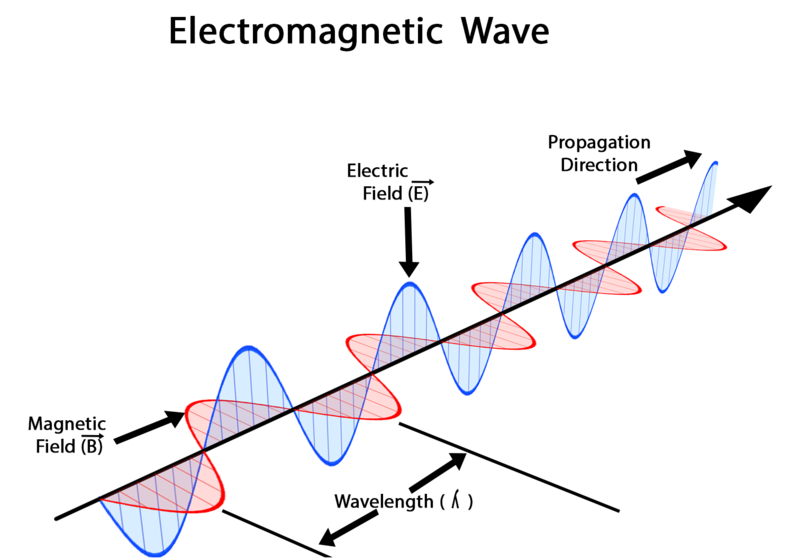
\includegraphics[width=\textwidth]{800px-Electromagnetic_waves.png}
\caption{Rappresentazione di un'onda elettromagnetica \cite[]{dechammaklKnnddRr2018}.}
\label{fig:Electromagnetic-waves}
\end{figure}

% \todo[inline]{Se c'è tempo: mostrare ``diagramma di Venn'' delle polarizzazioni, ci sono tre polarizzatori lineari, due di essi ortogonali e il terzo a \SI{45}{\degree} rispetto ad entrambi. Sono tutti a forma di cerchio, messi in modo tale da vedere tutte le possibili combinazioni. In questo modo, nell'intersezione dei due ortogonali si vede nero, mentre con tutti e tre si vede un po' di luce che passa.}

Questo ha delle applicazioni pratiche: ad esempio, gli occhiali che si usano per vedere i film 3D usano due lenti con filtri polarizzatori perpendicolari, una orizzontale e una verticale; in questo modo possono mostrare due immagini diverse ad ogni occhio.

\todo[inline]{Inserire tabella/grafico con le varie lunghezze d'onda della luce.}

A fine 1800 la questione della luce sembrava risolta, ma ben presto si scoprì un effetto che metteva i bastoni fra le ruote: l'\emph{effetto fotoelettrico}.

Detta in sintesi, la questione è questa: se si manda della luce su certi materiali si può ``eccitare'' i loro elettroni, ovvero strapparli agli atomi dei quali facevano parte.
La parte che non funziona con la teoria ondulatoria di Maxwell è il fatto che, mantenendo la stessa intensità di luce ma aumentandone la \emph{frequenza} l'energia cinetica degli elettroni strappati aumenta. 

Questo non sembra avere senso: stiamo mandando la stessa quantità di energia, e gli elettroni uscenti ne hanno di più? 
(Non c'è violazione della conservazione dell'energia: gli elettroni sono più energetici ma ce ne sono di meno).

Si scopre così che a ogni frequenza si può associare una energia caratteristica, e la relazione che lega energia e frequenza è \emph{lineare}! La relazione è 
%
\begin{align}
E = h f
\,,
\end{align}
%
dove \(E\) è l'energia caratteristica, \(f\) è la frequenza della luce, mentre 
%
\begin{align}
h = \SI{6.62607015e-34}{J / Hz}
\,,
\end{align}
%
è la costante di proporzionalità, che si chiama \textbf{costante di Planck}. 
Nota interessante: il valore è esatto dal 2018. Questo numero è così importante che definiamo le nostre unità di misura a partire da esso.

Cosa vuol dire ``energia caratteristica''? 
L'ipotesi avanzata da Einstein e Planck per spiegare l'effetto fotoelettrico e altri fenomeni, come la radiazione di corpo nero, fu quella che la luce fosse suddivisa in quanti indivisibili, che poi furono chiamati \textbf{fotoni}, caratterizzati proprio da un'energia data da \(E = hf\). 

Il grande scienziato Millikan nella sua \emph{Nobel lecture} del 1924
\autocite[]{millikanRobertMillikanNobel1924} parla così della teoria della luce quantizzata: 

\begin{quotation}
``It may be said then without hesitation that it
is not merely the Einstein equation which is having extraordinary success at
the moment, but the Einstein conception as well.

But until it can account for the facts of interference and the other effects
which have seemed thus far to be irreconcilable with it, we must withhold
our full assent.''
\end{quotation}

Era chiaro, dunque, che la teoria corpuscolare non poteva spiegare del tutto i fenomeni osservati, che hanno caratteristiche ondulatorie.

Non entreremo nel \emph{come}, ma questo problema si è effettivamente risolto qualche anno dopo con la teoria dell'elettrodinamica quantistica (QED), che ad oggi è la teoria accettata. 
Così per chiudere in bellezza (non da dire a lezione), ecco la Lagrangiana della QED:
%
\begin{align}
\mathscr{L} = - \frac{1}{4}  F_{\mu \nu } F^{\mu \nu }
+ \overline{\psi} \qty(i \slashed{\DD} -m ) \psi 
\,.
\end{align}

Descriviamo tuttavia qualche caratteristica della QED: 
\begin{enumerate}
    \item è una teoria \emph{quantistica}: il campo elettromagnetico è suddiviso in unità indivisibili;
    \item è una teoria \emph{relativistica}: si può usare per fare buone predizioni anche quando gli oggetti in gioco vanno a velocità vicine a quella della luce;
    \item quando il numero di fotoni in gioco è molto alto è una teoria ben approssimata da quella classica di Maxwell.
\end{enumerate}

\todo[inline]{Figura: diagramma di Venn delle teorie, a matrioska QED, teoria elettromagnetica, meccanica ondulatoria, ray optics \cite[fig. 1.0-1]{salehFundamentalsPhotonics}.}

\begin{enumerate}
    \item Ottica ``corpuscolare'', a raggi: funziona bene per il trattamento basilare di come funzionano le lenti, e in generale per trattare tutti i fenomeni per cui la lunghezza d'onda della luce è abbastanza piccola rispetto agli oggetti in gioco. 
    \item Ottica ondulatoria scalare: spiega interferenza, diffrazione, rifrazione. È un'approssimazione scalare della teoria elettromagnetica.
    \item Ottica elettromagnetica: spiega tutti i fenomeni ondulatori, più quelli di polarizzazione, e l'interazione della luce con la carica e la corrente elettrica.
    \item Ottica quantistica: si riduce, quando ci sono molti fotoni, all'ottica elettromagnetica classica. Un fenomeno che si spiega con la teoria quantistica ma non in quella classica è quello che vedremo in laboratorio!
\end{enumerate}

\section{Note di probabilità}

Un \emph{evento} \(A\) è qualcosa che possiamo misurare, ovvero qualcosa per cui è possibile determinare se è avvenuto o meno. 
Possiamo assegnare \textbf{probabilità} agli eventi: cosa questo significhi esattamente è un'importante questione filosofica.\footnote{Io propendo per la scuola Bayesiana per la quale la probabilità di un evento riflette la nostra credenza soggettiva che un evento possa accadere: la possiamo calcolare come il minimo delle quote alla quale saremmo disposti a scommettere sull'evento, aspettandoci di guadagnare, ovvero la quota per la quale ci attendiamo di avere gioco equo.}

Un'interpretazione diffusa è quella frequentista: la probabilità è la frazione di casi in cui avviene l'evento \(A\) diviso per i casi totali: 
%
\begin{align}
    \mathbb{P} (A) \overset{\text{def}}{=} \frac{N_A}{N _{\text{TOT}}}
    \,,
\end{align}
%
dove \(N_A\) è il numero di volte che ho visto l'evento \(A\), mentre \(N _{\text{TOT}}\) è il numero di volte in cui ho ripetuto l'esperimento.

Possiamo definire eventi combinati: ad esempio, chiamiamo \(A\cap B\) l'evento in cui sono avvenuti sia \(A\) che \(B\).
Qui lo abbrevierò in \(AB\), visto che non c'è pericolo di confusione.

Un altro esempio è \(A \cup B\) l'evento in cui è avvenuto almeno uno fra i due.

\subsection{Probabilità condizionata}

Un concetto importante in statistica e probabilità è quello di \textbf{condizionamento}: qual'è la probabilità che avvenga l'evento \(B\), se so che è avvenuto \(A\)? 
Questo si denota con \(\mathbb{P} (B | A)\), ed è semplice da calcolare in linea teorica: quello che abbiamo effettivamente fatto è di ridurre il nostro insieme totale di casi considerati da \(N _{\text{TOT}}\) a \(N_A\): quindi, avremo 
%
\begin{align} \label{eq:probabilita-condizionata}
\mathbb{P}(B | A) = \frac{N_{BA}}{N_A} = \frac{ N_{BA} / N _{\text{TOT}}}{N_A / N _{\text{TOT}}} = \frac{\mathbb{P}(AB)}{\mathbb{P}(A)}
\,,
\end{align}
%
dove con \(BA\) (\(= AB\), non è importante l'ordine) si intende l'evento che avvengano sia \(A\) che \(B\). 

\subsection{Eventi indipendenti}

Due eventi si dicono indipendenti se l'avvenire di uno non influenza l'avvenire dell'altro: possiamo fare uso del concetto appena definito per formalizzare ciò, scrivendo 
%
\begin{align}
\mathbb{P}(A) = \mathbb{P}(A | B) 
\qquad \text{e} \qquad
\mathbb{P}(B) = \mathbb{P}(B | A) 
\,.
\end{align}

Possiamo semplicemente prendere una delle due, e con la formula \eqref{eq:probabilita-condizionata} scriveremo 
%
\begin{align} \label{eq:probabilita-indipenenti}
\mathbb{P}(A) = \mathbb{P}(A | B) = \frac{\mathbb{P}(AB)}{\mathbb{P}(B)}
\iff
\mathbb{P}(AB) = \mathbb{P}(A) \mathbb{P}(B)
\,,
\end{align}
%
e visto che la scrittura che abbiamo ottenuto è simmetrica per scambio di \(A\) con \(B\) non ci serve fare il conto con l'altra espressione.

Questa formula è ciò che caratterizza gli eventi indipendenti: si dice che le probabilità si possono \emph{fattorizzare}; l'``e'' logico all'interno della descrizione dell'evento si può portare fuori e diventa un prodotto fra numeri se e solo se gli eventi sono indipendenti.

\section{Il nostro esperimento}

Questa sezione è presa principalmente dall'introduzione di \textcite{thornObservingQuantumBehavior2004}.

L'effetto fotoelettrico è molto suggestivo dell'esistenza del quanto di luce --- il \textbf{fotone} --- ma non è una prova conclusiva. Si può dimostrare che l'effetto potrebbe essere anche spiegato assumendo che il campo elettromagnetico sia un'onda classica, mentre il \emph{detector} è quantizzato, ovvero composto di particelle.

L'obiettivo che ci poniamo in queste ore è di comprendere e replicare un esperimento di Grangier del 1986, che dà un'evidenza sperimentale molto forte per il fatto che la luce sia effettivamente composta di particelle.

L'idea di base dell'esperimento è di ridurre molto l'intensità di un fascio di luce e farlo passare per un \emph{beam splitter} --- entreremo più nel dettaglio, per ora diciamo semplicemente che è un pezzo di plexiglass costruito in modo tale che la luce incidente abbia un'eguale probabilità di andare dritta o di deviare di un angolo retto quando lo incontra.

Mettiamo dei sensori corrispondenti alle due uscite, e andiamo a verificare che se vediamo il fotone da una parte, non lo vedremo dall'altra.

Ci sono diversi problemi con questa prima grezza descrizione dell'esperimento, ma iniziamo con le basi: quali sono le componenti dell'apparato sperimentale?

\subsection{Laser}

Questo è uno strumento che Grangier non aveva a disposizione, ma che ci facilita molto la vita. 
Un LASER --- Light Amplification by Stimulated Emission of Radiation --- sfrutta le proprietà di come la luce interagisce con gli atomi, si può dire ``risuonando'' con gli elettroni, per amplificare una frequenza di luce ben precisa.

Cosa significa ``risonanza'' (domanda per loro)? 
L'idea è che abbiamo un sistema che possiamo sollecitare periodicamente, ad esempio spingendo un bambino su un'altalena.
Diciamo di spingere sempre con la stessa forza, ma variamo la frequenza alla quale lo facciamo.

Se spingiamo con troppa frequenza, il bambino starà vicino al centro. Se spingiamo con troppo poca frequenza, dopo ogni spinta si stabilizzerà al centro.
C'è una frequenza ottimale alla quale possiamo spingere, se lo facciamo esattamente al momento giusto possiamo amplificare la vibrazione.

Riescono a emettere dunque quello che, nel modello classico ondulatorio, è proprio l'\emph{onda piana} che abbiamo visto, descritta dalla sinusoide.

\subsection{Beamsplitter}

Un beam-splitter sono essenzialmente due prismi incollati insieme.
L'interfaccia interna fra di essi soddisfa le proprietà che abbiamo visto nella sezione \ref{sec:newton-vs-huygens}; i beamsplitter tendenzialmente sono fatti in modo tale che i coefficienti siano molto vicini a 
%
\begin{align}
\mathcal{R} = \mathcal{T} = \frac{1}{2}
\,.
\end{align}

Visto che da entrambi i lati dell'interfaccia c'è lo stesso materiale, la legge di Snell si applica in modo molto semplice visto che \(n_1 = n_2 \), dunque non c'è deflessione.

\subsection{Detector e fotomoltiplicatori}

Come facciamo a rilevare i fotoni? 
In genere, i sensori che utilizziamo si basano sull'effetto fotoelettrico, ovvero sul fatto che il fotone che arriva ha dell'energia, e la può utilizzare per spostare della carica elettrica.
Finché abbiamo molta luce, come quando facciamo una fotografia, questo va bene. Se abbiamo un po' meno luce, possiamo allungare il tempo di esposizione, oppure avere una grande superficie che consideriamo.

Il problema è sempre il fatto che l'energia di un singolo fotone è molto piccola, quindi la strategia è generalmente quella di aspettare che ne arrivino tanti, anche se ne rileviamo una piccola frazione va bene.

Questo non va bene per noi! Se vogliamo investigare le proprietà del singolo fotone dobbiamo riuscire a rilevare una significativa porzione di essi.

Il modo di risolvere questo problema è tramite una \emph{valanga}.
Il nostro sensore è un sistema instabile, quando arriva un fotone lo destabilizza come un calcio su un nevaio: non saremmo in grado di vedere il singolo fotone, ma riusciamo facilmente a vedere la valanga.
Il nome del sensore è proprio ``\textbf{fotodiodo a valanga}''.

Le valanghe in montagna sono irreversibili; nel caso dell'elettronica invece c'è un modo di resettare tutto.
Questo si può fare velocemente, ma non è istantaneo: dopo ogni fotone rilevato c'è una finestra temporale nella quale, se ne arriva un altro, non lo sapremo. 

Inoltre, una caratteristica dei sistemi instabili è che ogni tanto scattano per qualche perturbazione ambientale, senza che ci sia stato un fotone. 
I conteggi dovuti a questo vanno sotto il nome di \textbf{dark count}.

È importante che questo dark count sia basso rispetto ai conteggi veri.

\subsection{Cosa vogliamo misurare}

Rendiamo più concreto il discorso: è utile definire la quantità 
%
\begin{align}
g^{(2)} = \frac{\mathbb{P}(\text{coincidenza})}{\mathbb{P}(\text{riflesso})\mathbb{P}(\text{trasmesso})}
\,,
\end{align}
%
dove le probabilità sono riferite alla nostra \emph{misura} dell'evento descritto: \(\mathbb{P} (\text{riflesso})\) è la probabilità che un certo fotone sia riflesso, e che lo rileviamo come tale; item per \(\mathbb{P}(\text{trasmesso})\), mentre per \(\mathbb{P}(\text{coincidenza})\) intendiamo la probabilità di osservare ``contemporaneamente'' (questo è impreciso, sarà chiarificato a breve) un fotone trasmesso e un fotone riflesso.

\todo[inline]{inserire schema dell'apparato ``semplificato'', senza gate}

Questa quantità sarà quella che permetterà di sintetizzare il risultato del nostro esperimento: segue il fatto fondamentale per capire le predizioni dei due modelli. 

Nel \textbf{modello classico}, ondulatorio, l'onda luminosa arriva sul detector con una qualche intensità \(I\). Questa potrebbe dipendere dal tempo, ma concretamente varia poco quindi assumiamo che sia constante.
In tal caso, quello che ci aspettiamo dal modello classico è che, a seconda di quant'è l'intensità incidente il detector abbia una qualche probabilità di attivarsi. 

Crucialmente, le probabilità di attivazione dei due detector sono indipendenti: l'onda arriva in modo continuo ad entrambi i detector, che ogni tanto si attivano, ma l'attivazione di uno non influenza l'attivazione dell'altro. 

Per quello che abbiamo visto (vedi equazione \eqref{eq:probabilita-indipenenti}) in questo caso possiamo fattorizzare: allora ci aspettiamo \(g^{(2)} = 1\). 

Si può mostrare che, nel caso più generale in cui l'intensità luminosa non è costante ma invece dipende dal tempo, vale la disuguaglianza \(g^{(2)} \geq 1\).

Nel \textbf{modello quantistico} invece, dobbiamo considerare i singoli fotoni, che sono \emph{indivisibili}: dunque, se un fotone viene rilevato da una parte non può essere rilevato dall'altra. Allora, in questo caso ci aspettiamo \(g^{(2)} \approx 0\); realisticamente, visto che come abbiamo menzionato esiste il dark count ci aspettiamo di vedere un numero poco più alto di 0.

Ad ogni modo, se troviamo qualcosa di vicino a 0 e molto minore di 1 saremo riusciti a falsificare l'ipotesi classica.

Abbiamo detto prima che possiamo calcolare le probabilità dividendo gli eventi favorevoli per gli eventi totali.

Quindi, per calcolare il valore di \(g^{(2)}\) dovremo calcolare le tre probabilità in gioco, utilizzando la solita formula. Chiamiamo \(N _{\text{TOT}}\) il numero totale di fotoni incidenti sul beamsplitter: allora avremo 
%
\begin{align}
g^{(2)} = \frac{N_{RT} / N _{\text{TOT}}}{(N_R / N _{\text{TOT}}) (N_T / N _{\text{TOT}})} = \frac{N_{RT} N _{\text{TOT}}}{N_R N_T}
\,,
\end{align}
%
e qui si pone il problema: il risultato dipende dal numero totale di fotoni che arrivano al detector, e che non possiamo calcolare! Se proviamo a sommare \(N_R\) e \(N_T\) avremo qualcosa che potrebbe essere molto più piccolo del numero dei fotoni incidenti, visto che a priori non sappiamo quant'è l'efficienza dei nostri detector.

Fortunatamente c'è una soluzione a questo problema, e per descriverla dobbiamo introdurre un altro pezzo dell'apparato.

\subsection{SPDC}

Questa è forse la parte più complessa dell'apparato, dal punto di vista della fisica necessaria a spiegarne il funzionamento.

Esistono dei particolari cristalli, chiamati \textbf{cristalli nonlineari}, che esibiscono il fenomeno della Spontaneous Parametric Down-Conversion.

Quando illuminiamo questi cristalli con una luce come quella di un laser, quasi la totalità della luce passa attraverso il cristallo, ma se guardiamo in una direzione ad un angolo di qualche grado da quella del laser vedremo della luce che arriva ad esattamente \emph{metà} della frequenza del laser, ovvero metà dell'energia, ovvero il doppio della lunghezza d'onda. 
Se guardiamo dall'altra parte del cristallo, rileveremo un fenomeno esattamente simmetrico.

Quello che succede, in termini quantistici, è che i fotoni del laser interagiscono con gli elettroni del cristallo e, talvolta, un fotone viene trasformato in due fotoni, ognuno con metà dell'energia del fotone iniziale.

Per dire una cosa molto sexy: questi fotoni sono \emph{entangled}, intrecciati, il che significa che la descrizione che ne facciamo come sistema quantistico non può essere scomposta in due descrizioni di sottosistemi senza perdere qualcosa. 

Per fugare dubbi di circolarità: la descrizione che diamo di questo fenomeno è quantistica perché è quella che funziona, ma non abbiamo bisogno di assumere la teoria quantistica della luce perché il nostro apparato sperimentale funzioni.
Se mettiamo dei detector agli angoli corretti, vedremo che rilevano fotoni contemporaneamente alla frequenza giusta da un lato e dall'altro molto di più di quello che accade se li spostiamo ad un angolo poco più in là. 

\begin{exo}[Rate atteso di conteggi]
Il laser che useremo avrà una potenza di circa \SI{50}{mW} e la luce emessa avrà una lunghezza d'onda di circa \SI{500}{nm}. 

Mettiamo un filtro attenuatore che attenui la luce di un fattore 10000, inoltre la SPDC capita solo a un fotone su \num{e7}. Quant'è il numero di fotoni al secondo che ci aspettiamo di vedere nel gate, se il detector ha un'efficienza del \SI{10}{\percent}?

(I numeri sono molto spannometrici, da aggiornare eventualmente)
\end{exo}


\subsection{Com'è fatto il nostro apparato}

% Il nostro apparato è costruito in modo tale da permetterci di avere un ``insieme universo'' ben definito nel calcolare le probabilità: se prendessimo il laser e lo puntassimo direttamente al beam splitter, potremmo vedere un certo numero di conteggi da una parte e dall'altra, e potremmo controllare quante volte abbiamo visto una coincidenza, ovvero un evento nel quale i detector sono scattati nello stesso momento (entro un margine di errore --- entreremo nel dettaglio sulle coincidenze).

% Tuttavia, senza controlli non sapremmo valutare se queste coincidenze siano quelle attese o meno: questo perché i nostri detectors hanno un certo rate di dark count, e non scattano sempre quando c'è un fotone.
% Senza sapere quanto è grande l'insieme universo, il numero totale di fotoni che avrebbero potuto essere stati visti, non possiamo sapere se il numero di coincidenze che vediamo sia compatibile con quello atteso per la teoria classica. 

In uscita del laser attacchiamo un cristallo nonlineare. 
Questo produce luce intrecciata; da uno dei due lati mettiamo direttamente un sensore, chiamato \textbf{gate}. 

Dall'altro lato mettiamo l'apparato descritto prima: beamsplitter, e i due sensori per i fotoni riflessi e trasmessi.

\todo[inline]{Inserire schema}

Ora abbiamo un grande vantaggio rispetto a prima: possiamo usare il detector di gate come controllo, ovvero il nostro ``insieme universo'' è costituito dalle volte in cui questo detector è scattato; il numero di volte che è scattato il gate, \(N_G\), diventa il nostro \(N _{\text{TOT}} \).

Nel fare il conto, tuttavia, dovremo considerare che se il nostro insieme universo è questo insieme ristretto, allora dobbiamo condizionare sul fatto che il gate sia scattato: otteniamo, allora, 
%
\begin{align}
g^{(2)} = \frac{\mathbb{P}(RT | G)}{\mathbb{P}(R|G) \mathbb{P}(T|G)}
\approx \frac{N_{RTG} N_G}{N_{RG} N_{TG}}
\,.
\end{align}

\subsection{Coincidenze}

Abbiamo quasi esaurito i problemi sperimentali, ma ne rimane ancora uno grosso: cosa intendiamo esattamente con ``concidenza''? 

I detector mandano i segnali che vedono ad un oggetto detto \textbf{timetagger}, che li riceve e digitalizza, convertendoli in un numero intero. Questo numero intero corrisponde al numero di ``tick'' di un suo orologio interno passati da quando è stato acceso e quando è arrivato il fotone.
La spaziatura temporale fra due ``tick'' è all'incirca di \SI{81}{ps}.
% (ovvero poco più di  2 centimetri-luce!).

Questo è un tempo così breve che riusciamo a distinguere dei fenomeni molto rapidi: vedremo la differenza temporale dovuta al fatto che i cammini della luce sono di lunghezze leggermente diverse, e una dispersione dovuta a fenomeni come le variazioni temporali intrinseche dei sensori, e i minimi ritardi dell'elettronica.

Ora, mostriamo un grafico ottenuto nel seguente modo: per ogni fotone visto dal detector ``gate'' al tempo \(t_G\), cerchiamo il più vicino temporalmente fra quelli riflessi, e chiamiamo il suo tempo \(t_R\). 
Ci segnamo il valore di \(t_R - t_G\), e ripetiamo questa operazione per ogni click del gate. 

Facciamo un istogramma di queste differenze di tempi: l'altezza di ogni barra rappresenta il numero di volte che abbiamo trovato quel valore.


Vediamo un fondo di rumore, e un distinto picco.

\begin{exo}[Picchi delle differenze nei tempi]
    Dove ti aspetti che sia centrato il picco dei valori di \(t_R - t_G\)? E il picco di \(t_T - t_G\)? 
    (Inserire foto dell'apparato con scala, in modo che si possano determinare i ritardi dovuti al tempo di viaggio della luce).
\end{exo}

% \todo[inline]{Inserire grafico}
% Questo non è centrato a \(t_R = t_G\).

Gli eventi che stanno nel picco sono quelli che possiamo considerare come coincidenze. 
Come si quantifica esattamente ``nel picco''? C'è sicuramente un grado di arbitrarietà nella scelta, ma questa andrà a influenzare esattamente dove tagliamo le code: il grosso della curva sarà preso.

Come troviamo le coincidenze triple? Ne abbiamo una quando allo stesso evento del gate corrisponde sia un fotone riflesso che uno trasmesso.

% \section{In laboratorio}

\printbibliography

\end{document}
